% Auto-generated SRG mini report
\documentclass[11pt]{article}
\usepackage{graphicx}
\usepackage{booktabs}
\usepackage{hyperref}
\graphicspath{{../figures/}}

\title{SRG multi-run comparison}
\author{SRG Chemical Computing Platform v6.1}
\date{\today}

\begin{document}
\maketitle

\section{Experimental settings}
\begin{verbatim}
Comparison runs:
runs/example_water_nacl_davies
runs/example_water_nacl_davies
\end{verbatim}

\section{Summary metrics}
% Auto-generated comparison table
\begin{table}[t]
  \centering
  \caption{Final energy and ionic strength by run.}
  \label{tab:srg_compare}
  \begin{tabular}{lrr}
    \toprule
    Run & Final energy & $I$ final / mol\,L$^{-1}$ \\
    \midrule
    example\\_water\\_nacl\\_davies & -346.2 & 0.09963 \\
    \bottomrule
  \end{tabular}
\end{table}


\section{Results narrative}
% Multi-run comparison — see metrics/summary_metrics.json
Compared 1 runs: example_water_nacl_davies.


\section{Figures}

\begin{figure}[htbp]
  \centering
  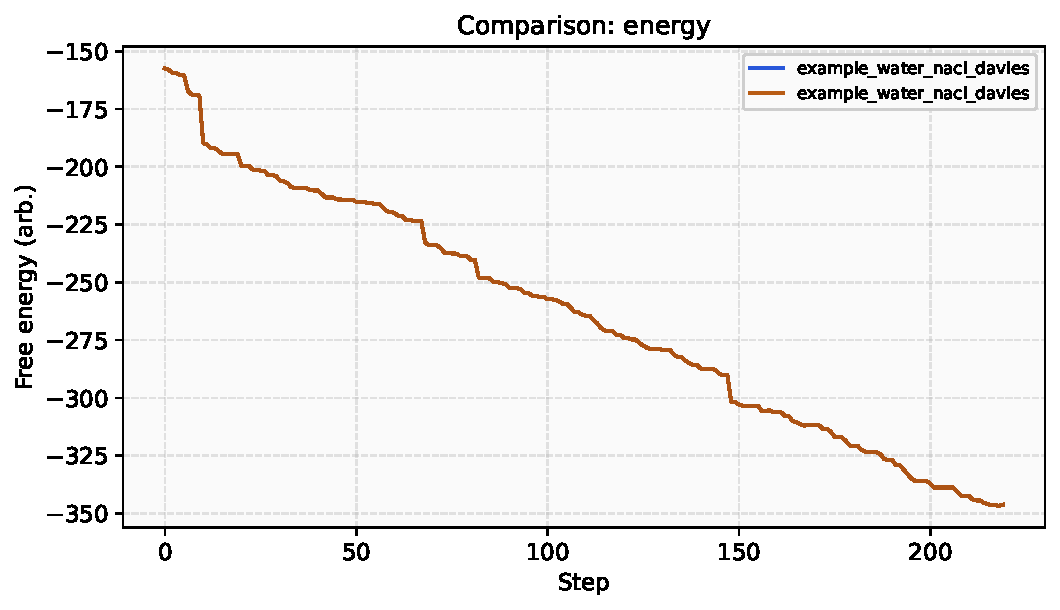
\includegraphics[width=0.92\linewidth]{fig_compare_energy.pdf}
  \caption{Figure: fig_compare_energy}
\end{figure}

\begin{figure}[htbp]
  \centering
  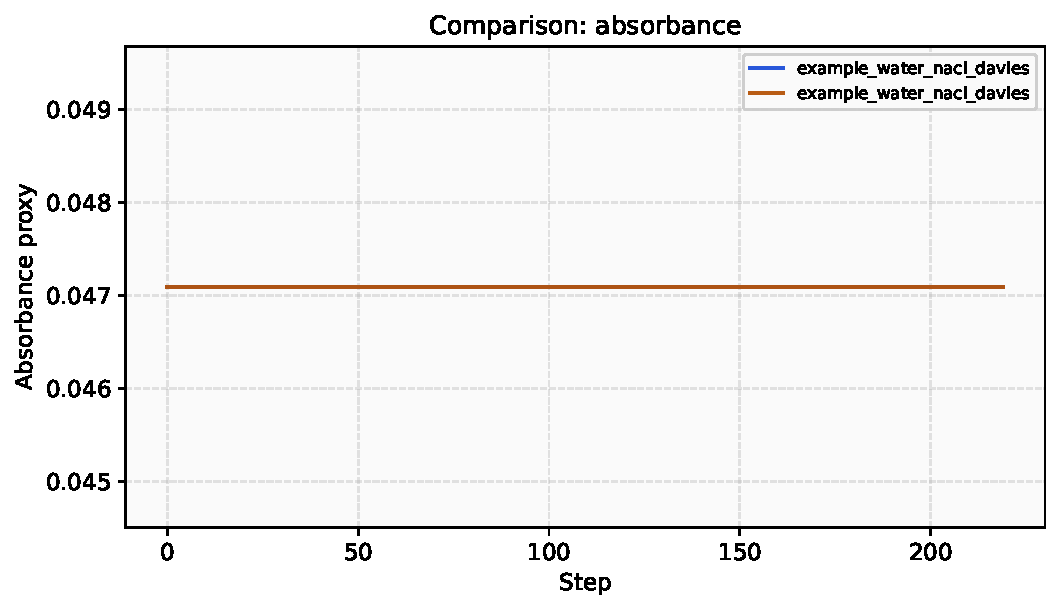
\includegraphics[width=0.92\linewidth]{fig_compare_absorbance.pdf}
  \caption{Figure: fig_compare_absorbance}
\end{figure}

\begin{figure}[htbp]
  \centering
  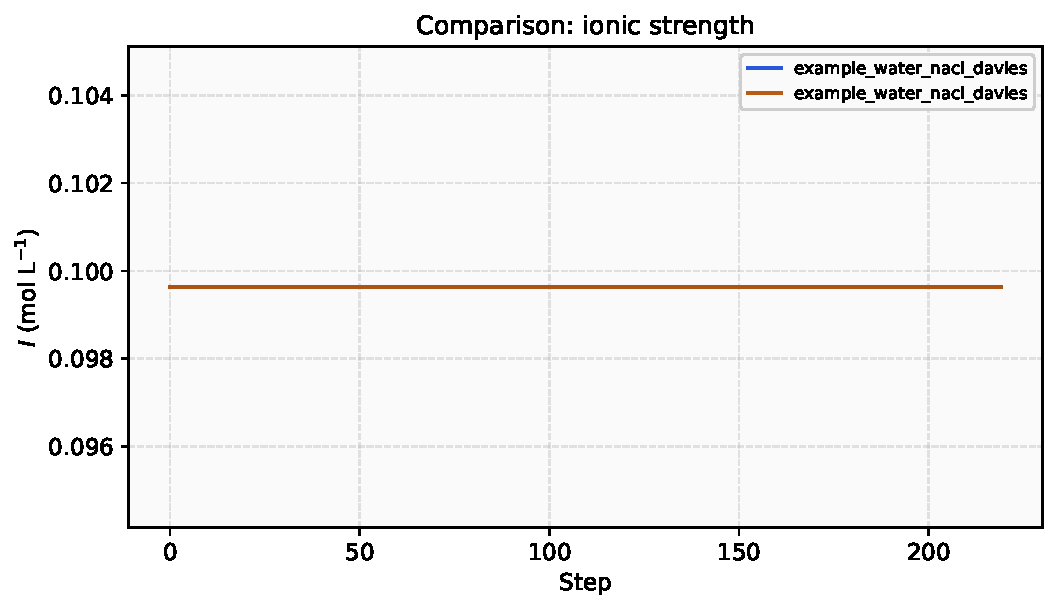
\includegraphics[width=0.92\linewidth]{fig_compare_ionic.pdf}
  \caption{Figure: fig_compare_ionic}
\end{figure}

\begin{figure}[htbp]
  \centering
  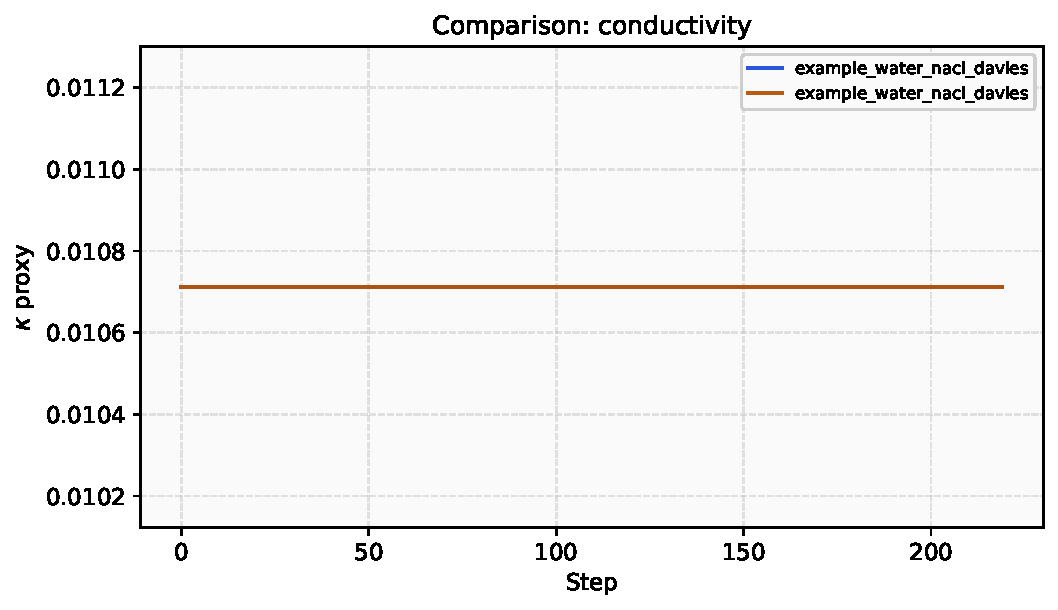
\includegraphics[width=0.92\linewidth]{fig_compare_conductivity.pdf}
  \caption{Figure: fig_compare_conductivity}
\end{figure}

\begin{figure}[htbp]
  \centering
  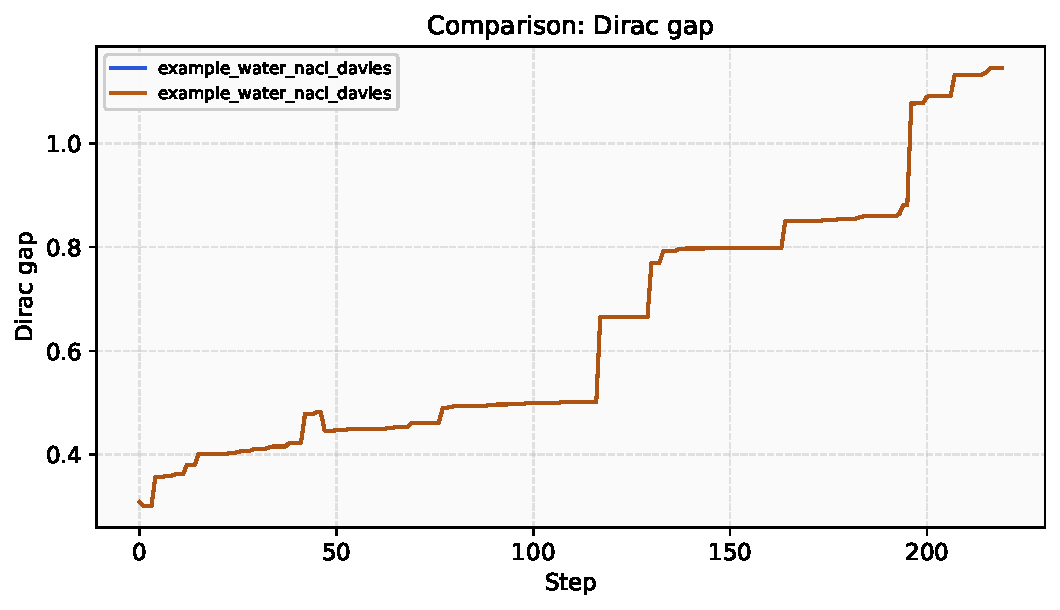
\includegraphics[width=0.92\linewidth]{fig_compare_spectral.pdf}
  \caption{Figure: fig_compare_spectral}
\end{figure}

\begin{figure}[htbp]
  \centering
  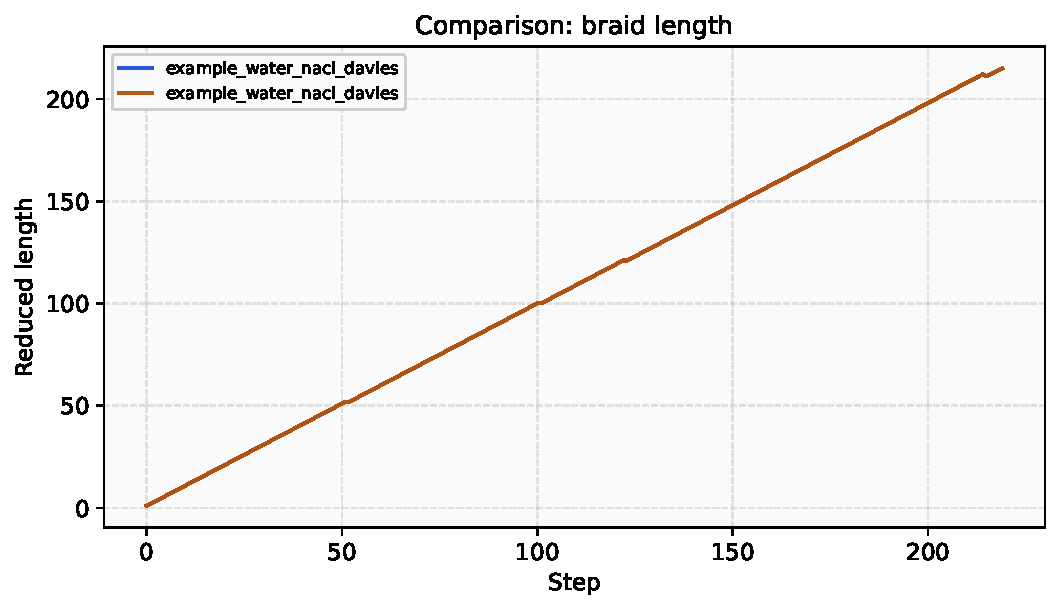
\includegraphics[width=0.92\linewidth]{fig_compare_braid.pdf}
  \caption{Figure: fig_compare_braid}
\end{figure}

\begin{figure}[htbp]
  \centering
  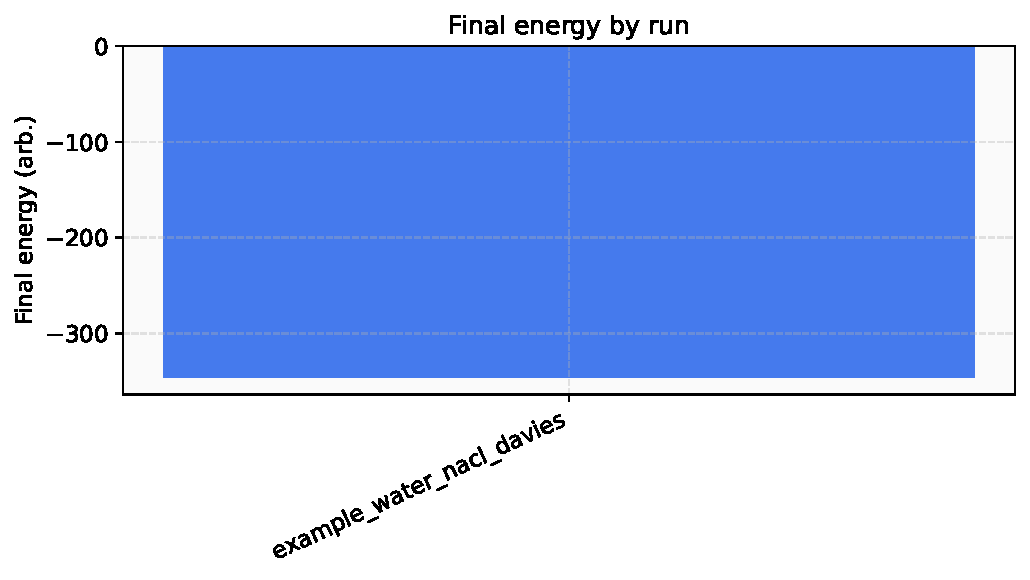
\includegraphics[width=0.92\linewidth]{fig_compare_bars.pdf}
  \caption{Figure: fig_compare_bars}
\end{figure}

\section{Interpretation}
The traces summarize coarse-grained graph energetics, optional electrolyte corrections,
spectral indicators from the discrete Dirac operator, and braid statistics on Monte Carlo moves.

\section{Limitations}
This MVP uses qualitative energy mappings and simplified DH/Davies/Pitzer proxies; it is not
a calibrated molecular simulation or experimental predictor.

\end{document}
